\subsection{Virtual PTZ camera}
Initially, some simple transformations were carried out in MATLAB using a symmetrical set of normalized homogeneous points, i.e. four points with coordinates (-1,-1,1), (1,-1,1), (1,1,1) and (-1,1,1) in $\mathbb{P}^2$.

Secondary trials were made with a point set with origo in a corner point, similar to the coordinate system in an image.
Here ``calibration'' matrices were needed in order to move the image origo to the center of the image and scale it.

Advancements into real-images were then straight forward as the synthezised calibration matrices were replaced with the real calibration matrices.
The resulting PTZ movement can be seen in fig. \ref{fig:ptz_res}.

\begin{figure}[H]
	\centering
	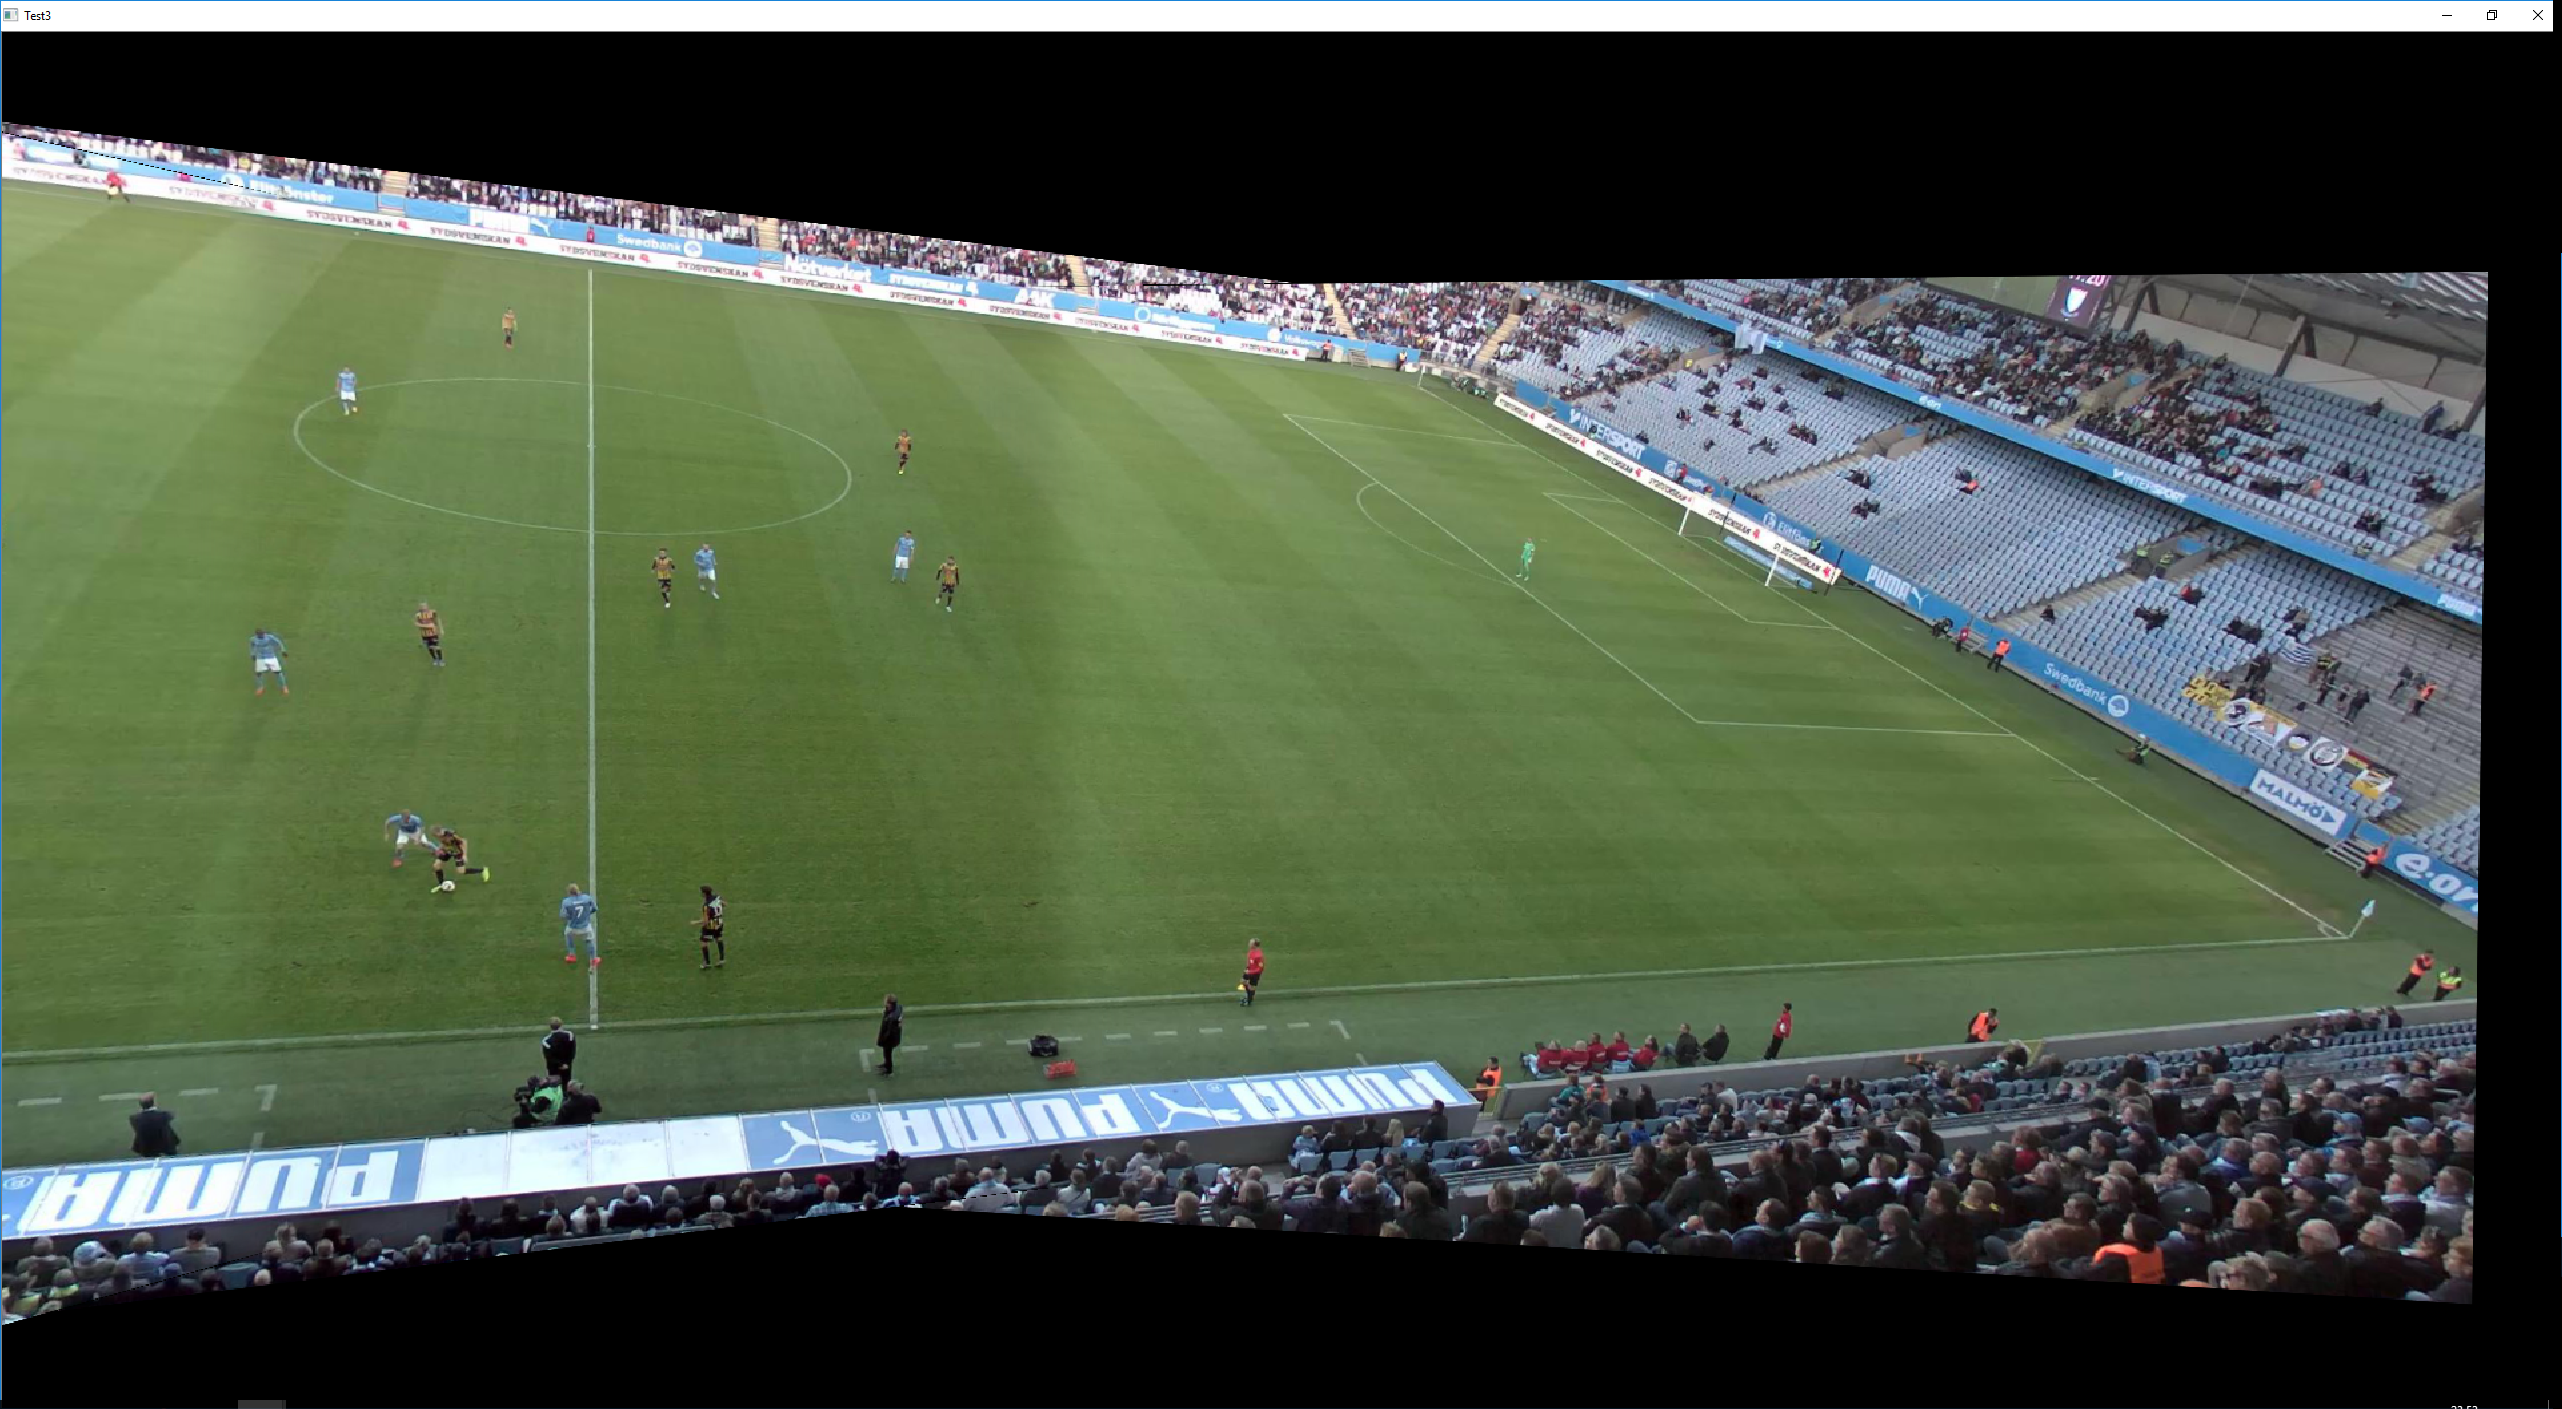
\includegraphics[width=0.8\columnwidth]{../results/images/PTZ_res.PNG}
	\caption{An example of the resulting image where the virtual camera has been panned, tilted and zoomed.}
	\label{fig:ptz_res}
\end{figure}
